\documentclass[fancy,blue,11pt]{elegantbook}

\title{An Elegant \LaTeX{} Template for Books}
\subtitle{Classic Elegant\LaTeX{} Template}

\author{Ethan Deng \& Liam Huang}
\institute{Elegant\LaTeX{} Program}
\date{\today}
\version{3.09}

\extrainfo{Victory won\rq t come to us unless we go to it. }

\logo{logo.png}
\cover{cover.jpg}

\begin{document}

\maketitle
\tableofcontents
\clearpage
\thispagestyle{empty}
\mainmatter
\hypersetup{pageanchor=true}

\chapter{Elegant\LaTeX{} Templates}
Elegant\LaTeX{} Program developers are intended to provide you beautiful, elegant, user-friendly templates. Currently, the Elegant\LaTeX{} is composed of \href{https://github.com/ElegantLaTeX/ElegantNote}{ElegantNote}, \href{https://github.com/ElegantLaTeX/ElegantBook}{ElegantBook}, \href{https://github.com/ElegantLaTeX/ElegantPaper}{ElegantPaper}, designed for typesetting notes, books, and working papers respectively. Latest releases are strongly recommended! This guide is aimed at briefly introducing the 101 of this template. For any other question, suggestion or comment, feel free to contact us on GitHub \href{https://github.com/ElegantLaTeX/ElegantBook/issues}{issues} or email us at \email{elegantlatex2e@gmail.com}.

Contact Infos:
\begin{itemize}
	\item Homepage: \href{https://elegantlatex.org/}{https://elegantlatex.org/}
	\item Github: \href{https://github.com/ElegantLaTeX/}{https://github.com/ElegantLaTeX/}
	\item CTAN: \href{https://ctan.org/pkg/elegantbook}{https://ctan.org/pkg/elegantbook}
	\item Wiki: \href{https://github.com/ElegantLaTeX/ElegantBook/wiki}{https://github.com/ElegantLaTeX/ElegantBook/wiki}
	\item Download: \href{https://github.com/ElegantLaTeX/ElegantBook/releases}{release}, \href{https://github.com/ElegantLaTeX/ElegantBook/archive/master.zip}{latest version}
	\item Weibo: ElegantLaTeX
	\item Wechat: ElegantLaTeX
	\item QQ: 692108391
	\item Email: \email{elegantlatex2e@gmail.com}
\end{itemize}


\section{ElegantBook Updates}
What\rq s new in this version:
\begin{enumerate}
   \item Remove \lstinline|\elegantpar|;
   \item Fix symbol font settings (by \href{muzimuzhi}{https://github.com/muzimuzhi});
\end{enumerate}

\begin{note}
	Since the latest version has witnessed huge reconstruction (with cover change in version 3.06), 3.x is backward incompatible with 2.x. For those who would like to convert documents compiled with earlier version (3.06 or 2.x) to be compatible with latest version, please refer to \href{https://github.com/ElegantLaTeX/ElegantBook/wiki/convert}{conversion}. Questions about version 2.x will not be answered henceforth.
\end{note}

\section{Installation and Update}
Both portable version and installation package are available for this template.

For portable version, simply download lastest ElegantBook-master from Github or CTAN (to be more accurate, download \lstinline{elegantbook.cls}) and save the file(s) under your working directory. This way of installation is simple and convenient, but you have to manually update \lstinline{cls} now and then.

If you are a \TeX{} Live 2019 user, using the \lstinline{tlshell}\footnote{namely, \TeX{} Live Manager} of \TeX{} Live 2019 direct installation package is strongly recommended. Simply search and open \lstinline{tlshell}, click on \lstinline{File -> Load Default Repository} or customize repository by \lstinline{Options}. Wait till the repository loads successfully, search \lstinline{elegantbook} by name, installation and update is just a click away.

\begin{figure}[htbp]
	\centering
	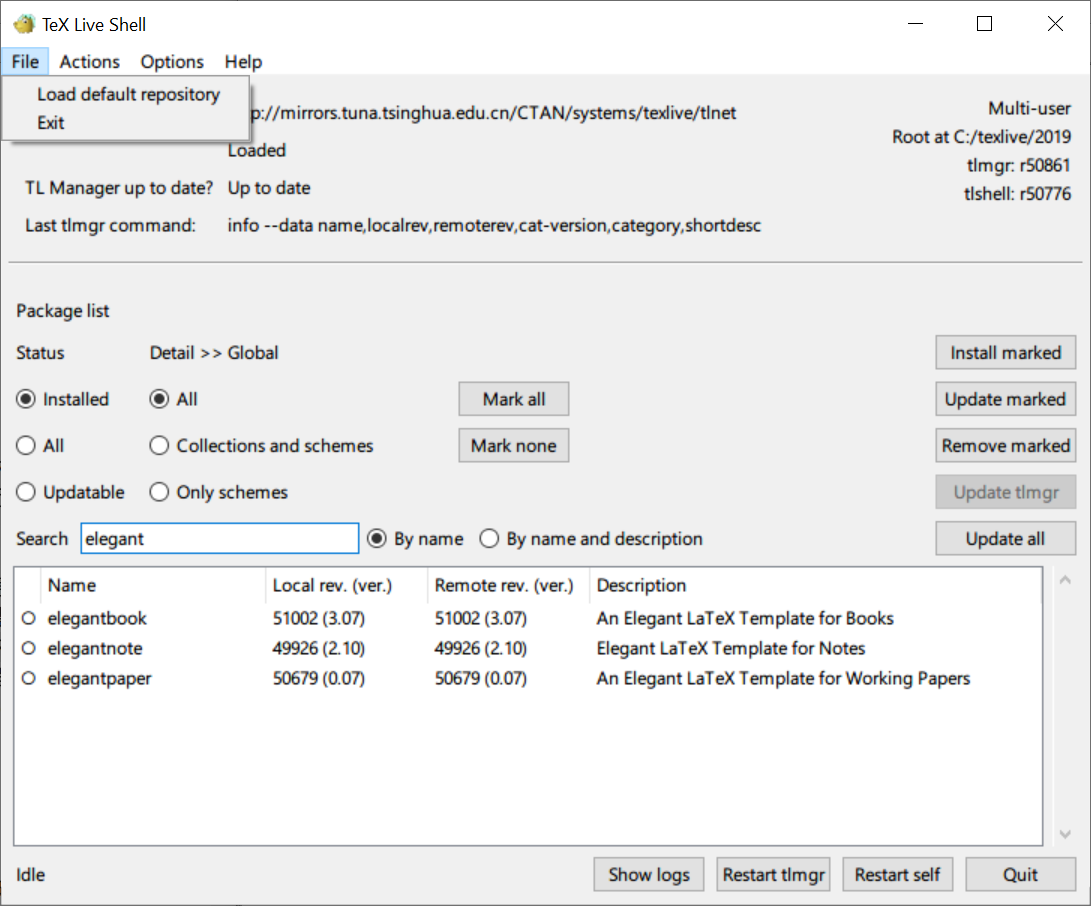
\includegraphics[width=0.7\textwidth]{tlshell.png}
	\caption{Use \TeX{} Live Shell to Install ElegantBook Template}
\end{figure}

If you are a \TeX{} Live 2018 user and would like to update to \TeX{} Live 2019, the official solution is to uninstall 2018. If you want to save the bother of uninstallation and installation, please copy \lstinline{elegantbook.cls} to the installation directory of \TeX{} Live 2018 (default: \lstinline|C:\texlive\2018\texmf-dist\tex\latex\elegantbook| ), run \lstinline{texhash} in cmd.

Excuse me? You are a  C\TeX{}  user? Sorry, this template is incompatible with C\TeX{}.

For more details about the installation and usage of \TeX{} Live 2019, the compatibility of C\TeX{} and \TeX{} Live, installation directory, etc., please refer to OG (Official Guide).

\section{Online Usage of Templates}
Considering the online usage of the templates, all the templates are available on Overleaf. Those who enjoy smooth network may feel free to use the templates without \TeX{} Live and to visit your documents anywhere anytime. Search \lstinline{elegantlatex} on Overleaf or visit \href{https://www.overleaf.com/latex/templates?addsearch=elegantlatex}{search result}, choose the one you prefer and save it to your account, then you can edit yourself or corporate with others if you like. For more infomation about Overleaf, please refer to Overleaf OG.

\section{User\rq s Selected Works Plan}
Eight years have passed since the found of Elegant\LaTeX{} Program. It\rq s an honor that our templates are preferred by a lot of users. Hence, in order to promote more interactions among our users and know more about what you need, we are planning to provide a platform to display selected works of our users on Github or our homepage. If you want to show us your work(s), contact us via Email or other ways. Or if you have upload your work(s) on Github or Gitee etc., share the URL(s) with us.

\section{About Pull Request}
For some reasons, pull request is unacceptable since May 20, 2019. For those who want to help revise the templates, submit issues or clone to your own repository to modify under the constriction of  LPPL-1.3c.

\section{Recruit Support Members}
Recruit Support Members for Elegant\LaTeX{} to translate template OGs(Chinese -> English), maintain wiki entries using MarkDown, update Wechat articles. No deadline for this recruitment.

Thank our best support members for their selfless work!
\begin{itemize}
	\item OG Translator: \href{https://github.com/peggy2006xzyz}{YPY};
	\item Wiki Maintainer: \href{https://github.com/izinngo}{Ingo Zinngo}, \href{Xiaohao890809}{https://github.com/xiaohao890809};
	\item QQ Group Manager: \href{https://github.com/sikouhjw}{Sikouhjw}.
\end{itemize}

\section{Acknowledgement}
The number of stars on Github for ElegantBook reached 100 on May 20, 2019 and was included in the \href{https://github.com/trending/tex?since=daily}{Trending} under the \TeX{} catagory. It is a remarkable moment for Elegant\LaTeX{} !!!

Thank China\TeX{} and \href{http://www.latexstudio.net/}{\LaTeX{} studio} for their promotion. \LaTeX{} studio offers tons of valuable posts and templates for discovery. It is the most comprehensive website on \LaTeX{} in China.

Thank muzimuzhi for the revision of the template.

If you like our template, star on Github.
\begin{figure}[htbp]
	\centering
	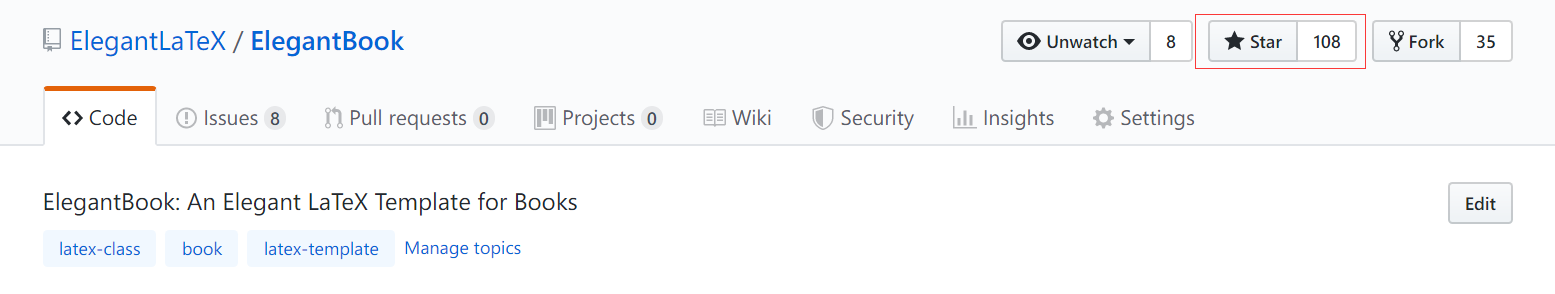
\includegraphics[width=\textwidth]{star.png}
	\caption{Twinkle, Twinkle, Little Star}
\end{figure}
Recently some users have expressed their love for our templates and want to tip us. QR code for donation is now available.
\begin{figure}[htbp]
	\centering
	
\includegraphics[width=0.5\textwidth]{donate.jpg}
\end{figure}

The explanation right of the tip usage belongs to Elegant\LaTeX{} with no supervision. Feel free to tip us. Those who donate more than 10 RMB will be recorded in the Donation List. Thank all the tippers!
\begin{table}[htbp]
	\centering
	\caption{Donation List}
	\begin{tabular}{cccc}
		\toprule
		Tipper   & Amount & Date & Channel \\
		\midrule
		Lerh  & 10 RMB  & 2019/05/15 & Wechat \\
		Yueguodipingxian & 10 RMB   & 2019/05/15 & Wechat \\
		Dapeng & 20 RMB & 2019/05/27 & Wechat\\
		Anonymous & 10 RMB & 2019/05/30 & Wechat \\
		\href{http://www.latexstudio.net/}{latexstudio.net} & 666 RMB & 2019/06/05 & Alipay \\
		Cassis & 11 RMB & 2019/06/30 & Wechat \\
		Anonymous & 10 RMB & 2019/07/23 & Wechat \\
		\bottomrule
	\end{tabular}%
\end{table}%

\chapter{ElegantBook Settings}

This template is based on the Standard \LaTeX{} book class, so the options of book class work as well. The default encoding is UTF-8 while \TeX{} Live is recommended. The test environment is Win10 + \TeX{} Live 2019. 


\section{Languages}
We defined one option named \lstinline{lang} which has two alternative values, \lstinline{lang=en} (default) and \lstinline{lang=cn}. Different values will alter the captions of figure/table, abstract name, refname, etc. You can use this option as
\begin{lstlisting}
\documentclass[en]{elegantbook} 
\documentclass[lang=en]{elegantbook}
\end{lstlisting}

\begin{remark}
Chinese Characters  are acceptable whenever \lstinline{lang=en} or \lstinline{lang=cn}. If you would like to include Chinese characters under (\lstinline{lstlisting}) environment, please use \lstinline{XeLaTeX} to compile.
\end{remark}

\section{Device Mode Option}
The option for device (\lstinline{device}) was originally used in ElegantNote, now we include this option in ElegantBook\footnote{Pictures have to be modified accordingly} as well. Activate iPad mode in the following way\footnote{Default size: normal, A4 paper}:
\begin{lstlisting}
\documentclass[pad]{elegantbook} %or
\documentclass[device=pad]{elegantbook}
\end{lstlisting}

\section{Color Themes}
This template contains 5 color themes, i.e. \textcolor{structure1}{\lstinline{green}}\footnote{Original default theme.}, \textcolor{structure2}{\lstinline{cyan}}, \textcolor{structure3}{\lstinline{blue}}(default), \textcolor{structure4}{\lstinline{gray}}, \textcolor{structure5}{\lstinline{black}}. You can choose \lstinline{green} with
\begin{lstlisting}
\documentclass[green]{elegantbook} %or
\documentclass[color=green]{elegantbook}
\end{lstlisting}


\begin{table}[htbp]
\caption{ElegantBook Themes\label{tab:color thm}}
\centering
\begin{tabular}{ccccccc}
\toprule
	        & \textcolor{structure1}{green} 
	        & \textcolor{structure2}{cyan} 
	        & \textcolor{structure3}{blue}
	        & \textcolor{structure4}{gray} 
	        & \textcolor{structure5}{black} 
	        & Main Environments\\
\midrule
structure & \makecell{{\color{structure1}\rule{1cm}{1cm}}}
				& \makecell{{\color{structure2}\rule{1cm}{1cm}}}
				& \makecell{{\color{structure3}\rule{1cm}{1cm}}} 
				& \makecell{{\color{structure4}\rule{1cm}{1cm}}} 
				& \makecell{{\color{structure5}\rule{1cm}{1cm}}} 
				& chapter  section  subsection \\
main      & \makecell{{\color{main1}\rule{1cm}{1cm}}}
				& \makecell{{\color{main2}\rule{1cm}{1cm}}}
				& \makecell{{\color{main3}\rule{1cm}{1cm}}}
				& \makecell{{\color{main4}\rule{1cm}{1cm}}}
				& \makecell{{\color{main5}\rule{1cm}{1cm}}}
				& definition  exercise  problem  \\
second    & \makecell{{\color{second1}\rule{1cm}{1cm}}}
				& \makecell{{\color{second2}\rule{1cm}{1cm}}}
				& \makecell{{\color{second3}\rule{1cm}{1cm}}}
				& \makecell{{\color{second4}\rule{1cm}{1cm}}}
				& \makecell{{\color{second5}\rule{1cm}{1cm}}}
				& theorem  lemma  corollary\\
third     & \makecell{{\color{third1}\rule{1cm}{1cm}}}
				& \makecell{{\color{third2}\rule{1cm}{1cm}}}
				& \makecell{{\color{third3}\rule{1cm}{1cm}}}
				& \makecell{{\color{third4}\rule{1cm}{1cm}}}
				& \makecell{{\color{third5}\rule{1cm}{1cm}}}
				& proposition\\
\bottomrule
\end{tabular}
\end{table}

If you want to customize the colors, please select \lstinline{nocolor} or use \lstinline{color=none} and declare the main, second, and third colors in the preamble section as follows:
\begin{lstlisting}[frame=single]
\definecolor{structurecolor}{RGB}{60,113,183}
\definecolor{main}{RGB}{0,166,82}%
\definecolor{second}{RGB}{255,134,24}%
\definecolor{third}{RGB}{0,174,247}% 
\end{lstlisting}


\section{Chapter Title Display Styles}

This template contains 2 sets of \textit{title display styles},\lstinline{hang}(default) and \lstinline{display} style. For the former, chapter title is displayed on a single line (\lstinline{hang}). For the latter, chapter title is displayed on a double line (\lstinline{display}).In this guide, we use \lstinline{hang} . To change display style
\begin{lstlisting}
\documentclass[hang]{elegantbook} %or
\documentclass[titlestyle=hang]{elegantbook}
\end{lstlisting}

\section{Theorem Class Environments}
We defined two sets of theorem modes, \lstinline{simple} style and \lstinline{fancy} style (default). You may change to \lstinline{simple} mode by

\begin{lstlisting}
\documentclass[simple]{elegantbook} %or
\documentclass[mode=simple]{elegantbook}
\end{lstlisting}

In this template, we defined four different theorem class environments

\begin{itemize}
\item \textit{Theorem Environment}, including title and content, numbering corresponding to chapter. Three types depending on the format:
   \begin{itemize}
      \item \textcolor{main}{\textbf{definition}} environment, the color is  \textcolor{main}{main};
      \item \textcolor{second}{\textbf{theorem, lemma, corollary}} environment, the color is \textcolor{second} {second};
      \item \textcolor{third}{\textbf{proposition}} environment, the color is \textcolor{third}{third}.
   \end{itemize}
\item \textit{Example Environments}, including \textbf{example, exercise, problem} environment, auto numbering corresponding to chapter.
\item \textit{Proof Environment}, including \textbf{proof, note} environment containing introductory symbol (\textbf{note} environment) or ending symbol (\textbf{proof} environment).
\item \textit{Conclusion Environments}, including \textbf{conclusion, assumption, property, remark, solution}\footnote{We also define an option \lstinline{result}, which can hide the \lstinline{solution} and \lstinline{proof} environments. You can switch between \lstinline{result=answer} and \lstinline{result=noanswer}} environment, all of which begin with boldfaced words, with format consistent with normal paragraphs.
\end{itemize}

\subsection{Theorem Class Environments}
Since the template uses the \lstinline{tcolorbox} package to customize the theorem class environments, it is slightly different from the normal theorem environments. The usage is as follows:
\begin{lstlisting}
\begin{theorem}{<theorem name>}{<label>}
The content of theorem.
\end{theorem}
\end{lstlisting}

The first parameter \lstinline{<theorem name>} represents the name of the theorem, and the second parameter \lstinline{label} represents the label used in cross-reference with \verb|ref{thm:label}|. Note that cross-references must be prefixed with \lstinline{thm:}. 

Other theorem class environments with the same usage includes:

\begin{table}[htbp]
   \centering
   \caption{Theorem Class Environments}
     \begin{tabular}{llll}
     \toprule
     Environment & Label text & Prefix & Cross-reference \\
     \midrule
     definition & label & def   & \lstinline|\ref{def:label}| \\
     theorem & label & thm   & \lstinline|\ref{thm:label}| \\
     lemma & label & lem   & \lstinline|\ref{lem:label}| \\
     corrlary & label & cor   & \lstinline|\ref{cor:label}| \\
     proposition & label & pro   & \lstinline|\ref{pro:label}| \\
     \bottomrule
     \end{tabular}%
   \label{tab:theorem-class}%
 \end{table}%
 

\subsection{Other Customized Environments}
The other three math environments can be called directly since there are no additional option for them, e.g. \lstinline{example}:
\begin{lstlisting}
\begin{example}
This is the content of example environment.
\end{example}
\end{lstlisting}

The effect is as follows:

\begin{example}
This is the content of example environment.
\end{example}

These are all similar environments with slight differences lies in:

\begin{itemize}
   \item Example, exercise, problem environments number within chapter;
   \item Note begins with introductory symbol and proof ends with ending symbol;
   \item Conclusion environment and so on are normal paragraph environments with boldfaced introductory words.
\end{itemize}

\section{Base Hide Option}
Hiding the end-of-chapter base is optional, simply type in:
\begin{lstlisting}
\documentclass[hide]{elegantbook} %or
\documentclass[base=hide]{elegantbook}
\end{lstlisting}


\section{Cover and Logo}

The cover image used in this template is from \href{https://pixabay.com/en/tea-time-poetry-coffee-reading-3240766/}{pixabay.com}\footnote{Thank China\TeX{} for providing free image source, \href{https://www.pexels.com/}{pexels.com} is strongly recommended.}. The image is completely free and can be used under any circumstance. The cover image size is $1280 \times 1024$. If you would like to change the cover, please crop it according to the size of the cover picture strictly.One free online image clipping site: \href{https://www.befunky.com/create/crop-photo/}{befunky.com}.

Aspect ratio of the logo is 1:1 in this guide, i.e. a square picture. To replace the logo, do remember to choose the appropriate picture.

\section{List Environments}
This template uses \lstinline{tikz} to customize the list environments, with \lstinline{itemize} environment customized to the third depth and \lstinline{enumerate} environment customized to fourth depth. The effect is as follows\\[2ex]
\begin{minipage}[b]{0.49\textwidth}
\begin{itemize}
   \item first item of nesti;
   \item second item of nesti;
   \begin{itemize}
      \item first item of nestii;
      \item second item of nestii;
      \begin{itemize}
         \item first item of nestiii;
         \item second item of nestiii.
      \end{itemize}   
   \end{itemize}
\end{itemize}
\end{minipage}
\begin{minipage}[b]{0.49\textwidth}
\begin{enumerate}
   \item first item of nesti;
   \item second item of nesti;
   \begin{enumerate}
      \item first item of nestii;
      \item second item of nestii;
      \begin{enumerate}
         \item first item of nestiii;
         \item second item of nestiii.
      \end{enumerate}   
   \end{enumerate}
\end{enumerate}
\end{minipage}

\section{Bibliography}

This template uses \hologo{BibTeX} to generate the bibliography, the default bibliography style is \lstinline{aer}. Let's take a glance at the citation effect. ~\cite{en1} use data from a major peer-to-peer lending marketplace in China to study whether female and male investors evaluate loan performance differently. 

If you want to use \hologo{BibTeX}, you must create a file named \lstinline{reference.bib}, add bib items (from Google Scholar, Mendeley, EndNote, and etc.) to \lstinline{reference.bib} file, then cite the bibkey in the \lstinline{tex} file. The Bib\TeX{} will automatically generate the bibliography for the reference you cited. If you want to add some noncited reference to the bibliography, you can use 
\begin{lstlisting}[frame=single]
\nocite{EINAV2010,Havrylchyk2018} %or include some bibitems
\nocite{*} %include all the bibitems
\end{lstlisting}

Two more options \lstinline{cite=numbers} and \lstinline{cite=authoryear} are available in this new version, with the default setting as \lstinline{numbers} since those major in science and technology use \lstinline{numbers} more often. For those who major in liberal arts want to use \lstinline{authoryear}, please type in:
\begin{lstlisting}
\documentclass[cite=authoryear]{elegantbook} %or
\documentclass[authoryear]{elegantbook}
\end{lstlisting}

\section{Preface}

If you want to add a preface before the first chapter with the number of chapter unchanged, please add the preface in the following way:
\begin{lstlisting}
\chapter*{Preface}
\addcontentsline{toc}{chapter}{Preface} 
\markboth{Preface}{} 
The content of Preface.
\end{lstlisting}

\section{Introduction Environment}
We create a introduction environment to display the structure of chapter. The basic useage is as follows
\begin{lstlisting}
\begin{introduction}
	\item Definition of Theorem
	\item Ask for help
	\item Optimization Problem
	\item Property of Cauchy Series
	\item Angle of Corner
\end{introduction}
\end{lstlisting}
you will get:
\begin{introduction}
	\item Definition of Theorem
	\item Ask for help
	\item Optimization Problem
	\item Property of Cauchy Series
	\item Angle of Corner
\end{introduction}

You can change the title of this environment by modifying the optional argument of this environment
\begin{lstlisting}
\begin{introduction}[Brief Introduction]
...
\end{introduction}
\end{lstlisting}

\section{Problem Set}
The environment \lstinline{problemset} is used at the end of each chapter to display corresponding exercises. Just type in the following sentences:
\begin{lstlisting}
\begin{problemset}
	\item exercise 1
	\item exercise 2
	\item exercise 3
\end{problemset}
\end{lstlisting}
And you will get:
\begin{problemset}
	\item exercise 1
	\item exercise 2
	\item exercise 3
\end{problemset}
\begin{remark}
If you want to customize the title of  \lstinline{problemset}, please change the optional argument like introduction environment.
\end{remark}


\chapter{ElegantBook Writing Sample}

\begin{introduction}
\item Theorem Class Envrionments
\item Cross Reference
\item Math Environments
\item List Environments
\item Logo and Base 
\item $a^2+b^2=c^2$
\end{introduction}


\lipsum[1]
% source: https://www.maths.tcd.ie/~dwilkins/LaTeXPrimer/Theorems.html

\section{Writing Sample}

We will define the integral of a measurable function in three steps. First, we define the integral of a nonnegative simple function. Let $E$ be the measurable set in $\mathcal{R}^N$.

\begin{definition}{Left Coset}{}
Let $H$ be a subgroup of a group~$G$.  A \emph{left coset} of $H$ in $G$ is a subset of $G$ that is of the form $xH$, where $x \in G$ and $xH = \{ xh : h \in H \}$. Similarly a \emph{right coset} of $H$ in $G$ is a subset of $G$ that is of the form $Hx$, where $Hx = \{ hx : h \in H \}$ $\hbar$
\end{definition}

\begin{note}
Note that a subgroup~$H$ of a group $G$ is itself a left coset of $H$ in $G$.
\end{note}

\lipsum[2]

\begin{theorem}{Lagrange's Theorem}{}
Let $G$ be a finite group, and let $H$ be a subgroup of $G$.  Then the order of $H$ divides the order of $G$.
\end{theorem}

\lipsum[3]

   
\begin{proposition}{Size of Left Coset}{}
Let $H$ be a finite subgroup of a group $G$.  Then each left coset of $H$ in $G$ has the same number of elements as $H$.
\end{proposition}

\begin{proof}
Let $z$ be some element of $xH \cap yH$.  Then $z = xa$ for some $a \in H$, and $z = yb$ for some $b \in H$. If $h$ is any element of $H$ then $ah \in H$ and $a^{-1}h \in H$, since $H$ is a subgroup of $G$. But $zh = x(ah)$ and $xh = z(a^{-1}h)$ for all $h \in H$. Therefore $zH \subset xH$ and $xH \subset zH$, and thus $xH = zH$.  Similarly $yH = zH$, and thus $xH = yH$, as required.
\end{proof}

\begin{figure}[htbp]
	\centering
	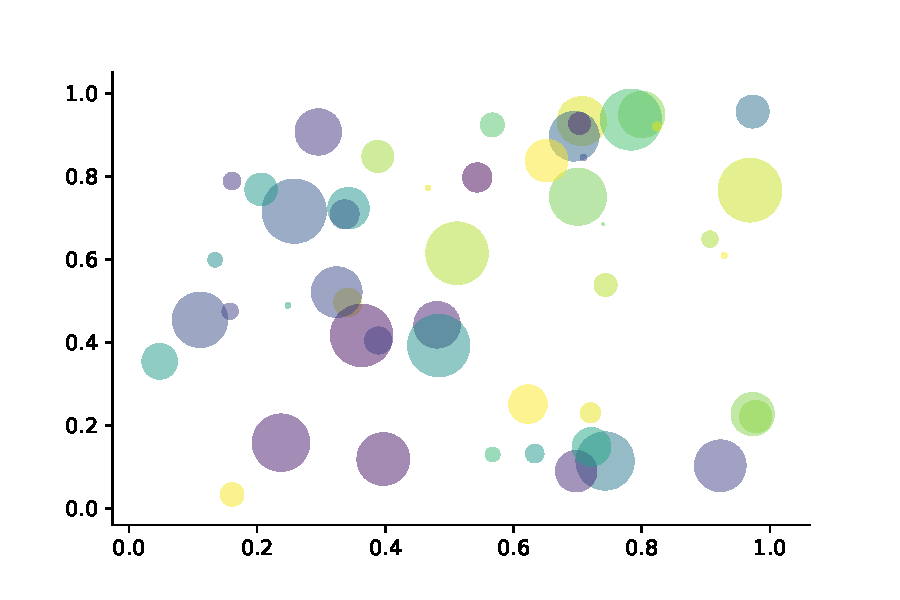
\includegraphics[width=0.6\textwidth]{scatter.pdf}
	\caption{Matplotlib: Scatter Plot Example\label{fig:scatter}}
\end{figure}

Regression analysis is a powerful statistical method that allows you to examine the relationship between two or more variables of interest. While there are many types of regression analysis, at their core they all examine the influence of one or more independent variables on a dependent variable. The process of performing a regression allows you to confidently determine which factors matter most, which factors can be ignored, and how these factors influence each other.

Let's continue using our application training example. In this case, we'd want to measure the historical levels of satisfaction with the events from the past three years or so, as well as any information possible in regards to the independent variables. 


\begin{table}[htbp]
  \small
  \centering
  \caption{Auto MPG and Price \label{tab:reg}}
    \begin{tabular}{lcc}
    \toprule
                    &       (1)         &        (2)      \\
    \midrule
    mpg             &    -238.90***     &      -49.51     \\
                    &     (53.08)       &      (86.16)    \\
    weight          &                   &      1.75***    \\
                    &                   &      (0.641)    \\
    constant        &     11,253***     &       1,946     \\
                    &     (1,171)       &      (3,597)   \\
    obs             &        74         &         74     \\
    $R^2$           &      0.220        &       0.293    \\
    \bottomrule
    \multicolumn{3}{l}{\scriptsize Standard errors in parentheses} \\
    \multicolumn{3}{l}{\scriptsize *** p<0.01, ** p<0.05, * p<0.1} \\
    \end{tabular}%
\end{table}%

\lipsum[1-2]

\begin{itemize}
	\item Routing and resource discovery;
	     \begin{itemize} 
      	   	\item Language Models
       	 	\item Vector Space Models
    		 \end{itemize}
	\item Resilient and scalable computer networks;
	\item Distributed storage and search.
\end{itemize}

\begin{problemset}
	\item Solve the equation $5(- 3x - 2) - (x - 3) = -4(4x + 5) + 13$.
	\item Find the distance between the points (-4 , -5) and (-1 , -1). 
	\item Find the slope of the line $5x - 5y = 7$.
\end{problemset}


\chapter{FAQ}

\begin{custom}{Question}
	I want to customize font and background color.
\end{custom}

\begin{solution}
	Please use \lstinline{\pagecolor} to change background color, refer to \href{https://tex.stackexchange.com/questions/278544/xcolor-what-is-the-equivalent-of-default-text-color}{this} to customize font.
\end{solution}



\begin{custom}{Question}
	Which version should I choose?
\end{custom}

\begin{solution}
	Please use \href{https://github.com/ElegantLaTeX/ElegantBook/releases}{Latest Release} via GitHub or \TeX{} Live 2019.
\end{solution}


\begin{custom}{Question}
	Which editor should I choose?
\end{custom}

\begin{solution}
	You can use \TeX{} Live 2019 built-in \TeX works or \TeX Studio. You may refer to \href{https://github.com/EthanDeng/texworks-autocomplete}{\TeX{}works autocomplete}. \TeX{} Live 2019 + \TeX{}studio is strongly recommended. I myself use VS Code and Sublime Text. Related configurations can be found at \href{https://github.com/EthanDeng/vscode-latex}{vscode-latex} and \href{https://github.com/EthanDeng/sublime-text-latex}{sublime-text-latex}.
\end{solution}


\begin{custom}{Question}
	Hello, we want to use ElegantBook to write a book about machine learning and would like your authorization.
\end{custom}

\begin{solution}
	Feel free to use our templates by pointing out our copyright. For other issues, please refer to LPPL-1.3c. If you want to show us your work, share the URL with us afterwards.
\end{solution}

\begin{custom}{Question}
	I would like to use the former cover!
\end{custom}

\begin{solution}
	Cover option is forthcoming.
\end{solution}



\begin{custom}{Question}
	What is cross reference?
\end{custom}

\begin{solution}
	This template is aimed at who are not a complete beginner for \LaTeX{}. Please learn more about \LaTeX{} before using this template.
\end{solution}


\begin{custom}{Question}
	Is the language for code highlighting optional?
\end{custom}

\begin{solution}
	Yes, \lstinline{listings} package is used in ElegantBook, hence language is optional. For global setting, use \lstinline{\lstset}. For more information, please refer to package documentations.
\end{solution}


\nocite{en1,en2,en3} 
\bibliography{reference}

\appendix
\chapter{Mathematical Tools}

This appendix covers some of the basic mathematics used in econometrics. We briefly discuss the properties of summation operators, study the properties of linear and some nonlinear equations, and review the ratios and percentages. We also introduce some special functions that are common in econometrics applications, including quadratic functions and natural logarithms. The first four sections require only basic algebraic techniques. The fifth section briefly reviews differential Calculus Although Calculus is not necessary to understand much of this book, it is used in some of the end-of-chapter appendices and in some of the more advanced topics in part 3.

\section{Summation Operator and Description Statistics}

\textbf{Summation Operator} is an abbreviation used to express the summation of numbers, it plays an important role in statistics and econometrics analysis. If $\{x_i: i=1, 2, \ldots, n\}$ is a sequence of $n$ numbers, the summation of the $n$ numbers is:

\begin{equation}
\sum_{i=1}^n x_i \equiv x_1 + x_2 +\cdots + x_n
\end{equation}

\chapter{A Minimal Example}

\begin{lstlisting}[frame=single]
\documentclass{elegantbook}
% title info
\title{Title}
\subtitle{Subtitle is here}
% bio info
\author{Your Name}
\institute{XXX University}
\date{\today}
% extra info
\version{1.00}
\extrainfo{Victory won\rq t come to us unless we go to it. --- M. Moore}
\logo{logo.png}
\cover{cover.jpg}

\begin{document}

\maketitle
\tableofcontents
\mainmatter
\hypersetup{pageanchor=true}
% add preface chapter here if needed
\chapter{Example Chapter Title}
The content of chapter one.

\bibliography{reference}
\end{document}
\end{lstlisting}


\end{document}
